\documentclass{llncs}
\usepackage[ruled,vlined]{algorithm2e}
\usepackage{color,graphicx,epstopdf,changepage,amsmath,multirow}

\SetAlgoCaptionSeparator{.\space}
\renewcommand\AlCapFnt{\normalfont\scshape}
\setlength{\algomargin}{0.7cm}

\title{A Novel Comprehensive Quality Evaluation Model in Automated Semantic Web Service Composition}

\author{Chen Wang, Hui Ma, and Aaron Chen}
\institute{School of Engineering and Computer Science,
\\Victoria University of Wellington, New Zealand \\
\email{\{Chen.Wang, Hui.Ma, and Aaron.Chen\}@ecs.vuw.ac.nz }}

\makeatletter
\usepackage[pdfauthor={\@author}, pdftitle={\@title}]{hyperref}
\makeatother

\providecommand{\e}[1]{\ensuremath{\times 10^{#1}}}

\begin{document}

\maketitle

\begin{abstract}
Semantic web service composition has been a prevailing research area in recent years. There are two major governance challenges faced by researchers, and Semantic matchmaking is to discover interoperable web services, which demands a rich “machine understanding” language such as OWL-S (Web Ontology language for Web Services), WSML (Web Service Modeling language, SAWSDL (Semantic Annotations for WSDL and XML Schema). This interaction enables us to pair service functionalities through language understanding and reasoning. An optimisation problem is the another challenge with consideration in non-functional attributes, such as quality of service (QoS). Nowadays, many scholars have looked into optimisation problems in QoS-awareness web service composition applying AI planning and Evolution Computing techniques. However, it is not sufficient without considering good balancing between functional and nonfunctional quality in most scenarios. Therefore, the consideration in these two quality dimensions is a must, so that a comprehensive quality evaluation model is proposed to deal with finding optimised semantic web service composition solution. This paper develops a more applicable approach dealing with a comprehensive quality ---semantic matchmaking and QoS optimisation for automated semantic web service composition.
\end{abstract}

\section{Introduction}\label{introduction}
Service-oriented computing (SOC) is a novel computing paradigm that employs services as fundamental elements to achieve agile development of cost-efficient and integratable enterprise applications in heterogeneous environments \cite{papazoglou2003service}. Service Oriented Architecture (SOA) could abstractly realise service-oriented paradigm of computing, this accomplishment has been contributing to reuse of software components, from the concept of functions to units and from units to services during the development in SOA \cite{booth2004web}. One of the most typical realisations of SOA is \textit{web service}, which designated as ``modular, self-describing, self-contained applications that are available on the Internet'' \cite{curbera2001web}. Several standards play a significant role in registering, enquiring and grounding web services, such as UDDI, WSDL and SOAP \cite{fensel2011semantic}.

\textit{Web service composition} pertains to a combination of several web services to provide a value-added composite service that accommodates customers' arbitrarily complex requirements. This application is developed by integrating interoperable and collaborative functionalities over heterogeneous systems - diverse platforms and programming languages \cite{casati2001technologies}. Due to an increase in a large-scale alignment of enterprise applications, the number of Web services has increased dramatically and unprecedentedly, which cause an immense redundancy in functionality in a huge searching space. Therefore, manual service and semi-automated web service composition are considered to be lower efficiency while automated web service composition is considered to be less human intervention, less time consumption, and high productivity.

Two most notable challenges for web service composition are ensuring interoperability of services and QoS optimisation \cite{fensel2011semantic}. Interoperability of web services is one challenge in the dimensions of syntactic and semantics \cite{fensel2011semantic}. The syntactic dimension has achieved success through the use of XML standards (such as $WSDL$, $SOAP$), the semantics dimension, on the other hand, demands further research. Adding semantics given by ontologies \cite{o2005review} enables web service to understand and reason with each other. Historically, there are many ontologies languages and formats for semantic service descriptions, such as OWL-S \cite{martin2004owl}, WSML \cite{fensel2006enabling}, and SAWSDL \cite{lausen2007semantic}, The logical characteristics in reasoning makes ``machine understanding'' possible through identifying and matching semantic similarity in input/output parameters of web services in heterogeneous environments. The second challenge is to find optimised solutions to Quality of Service ($QoS$) over the composite web service. This problems give birth to \textit{QoS-aware service composition} that considers the composition of service-level agreements \cite {sahai2002automated} manifesting a collection of SLA rules and policies for supporting QoS-based composition.

Existing works on service composition are often addressed regarding one of the above challenges. One group optimises the quality of compositions under a pre-defined abstract workflow, which is considered to be a \textit{semi-automated Web service composition} approach. Another group attempts to generate a composite plan automatically in discovering and selecting suitable web services, which are deemed to be an NP-hard problem \cite{moghaddam2014service}. \textit{Semantic web services composition} is distinguished from the syntactic service composition. Its benefits are presented in eliminating conflicts at the semantic level of web service composition. In the last few years, substantial work has been done on semantic web service composition \cite{fensel2011semantic,lecue2009optimizing}. Howevever, few works have addressed an automatic semantic web service composition approach, which optimise both QoS and quality of semantic matchmatching as optimised web service composition sollutions. For example, customers prefer the highest quality of service solution associated with the acceptable semantic matchmatching quality.

The overall goal of this paper is to develop an comprehensive evaluation model in  automated semantic web service composition that satisfactorily optimises both functional and non-functional requirements. Particularly, this project considers a semantic matchmaking quality extension to QoS awareness and a few structural constructs(sequence and parallel) for building optimised composition solution using Particle Swarm Optimisation. We aim to provide a more general and applicable way to measure semantic matchmaking in automated semantic web service composition and contribute to the state-of-the-art in this field. Three objectives of this work are accomplished as follows:

\begin{enumerate}
 \item To address semantic matchmaking quality with considering different matching types associated with corresponding semantic similarity, which is demonstrated as a comprehensive quality --- a more general and applicable evaluation method utilising semantic information of service descriptions in this paper.
 
 \item To apply PSO for sorting an optimised service queue as a indirect representation of web service composition with consideration in optimising the comprehensive quality, this indirect representation is decoded using graph building algorithm to generate a service composite solution.
  
 \item To evaluate the performance of proposed approaches, we utilise the datasets from Web Services Challenge 2009 (WSC09) \cite{kona2009wsc}.
\end{enumerate}

The remains of this paper are composed as the following: Sect. \ref{background} provides the knowledge background on the semantic web service composition, including a literature review; Sect. \ref{qswsc_approach} represents the an Introduction of of semantic automated web service composition approach, and the comprehensive quality evaluation model; Sect. \ref{experiment_design} describes the experiments conducted to test the effectiveness of proposed model; Sect. \ref{results_analysis} presents the results and analysis of these experiments; Sect. \ref{conclusion} is the paper conclusion.


\section{Background}\label{background}

\subsection{Problem Description}\label{problemDes}

The purpose of web service composition is to accomplish an arbitrarily complex task fulfilling customer's requirement, which could be denoted as composite goal: $Comp.G(F(T_{Input}, T_{Output}), NF(T_{QoS}))$. This overall composite goal is demonstrated in two parts. One part is that a given input or input set to get the desired output or output set, it typically refers to a statement in functional requirement ; another part specify the overall acceptable composite quality, which covers aspects in non-functionality. To accomplish the first half goal, two stages are involved in the investigation of this paper : services discovery and service selection. Firstly, service discovery is to find matched web service: $S_{n}(F(S_{Input}, S_{Output}), NF(S_{QoS}))$ from Service Repository: $S \{S_{1}, S_{2},..., S_{n} \}$ with the given Task until the desired output found. It results in more than one solutions without considering optimisation; Service selection is to select web services to reach global best quality($T_{QoS}$). We are aiming to optimise a combined objective function involving both functional and non-functional concerns. Particularly in this paper, two challenges mentioned in Sect. \ref{introduction} are addressed in semantic web composite approach. First, the inputs of each service could be semantically matched by predecessor services in the composition. Second, optimisation in QoS would not be sufficient in many scenarios to make a good decision, if customers are looking for a trade off either in better service quality with counteroffer in QoS or better QoS with less strict functional matchmaking quality.

\subsection{Semantic Web Service matchmaking Type}\label{semantic Web service Discovery}
The semantic service matchmaking aims to discover appropriate services from service repository relevant to a customer's functional request defined by the Goal. A semantic web service is defined by $S(F(S_{Input}\in C_{1}, S_{Output}\in C_{2}), NF(S_{QoS}))$ with both Input and Output are linked to concept $C_{1}$ and $C_{2}$ in an ontology ($O$) respectively, satisfying $O=\{C, Tax\}$. The web service discovery process is to discovery the services an input-output concept matchmaking according to the Taxonomy(Tax) within an ontology (O). To measure the quality of semantic matchmaking, different matching levels that are typically considered in the literature \cite{paolucci2002semantic}. We defined two web services associated with parameters in a particular domain: $S_{1}$ $(F(S_{Input}\in C_{1}, S_{Outputs}\in C_{2}), NF(S_{QoS}))$ and  $S2$ $(F(S_{Input}\in C_{3}, S_{Output}\in C_{4}), NF(S_{QoS}))$ and an Ontology($O$) with $C_{1},C_{2},C_{3}$, and $C_{4}$ defined in. 

\begin{itemize}
\item \textit{Exact} ($\equiv$): Output of Web service $S_{1}$ and Input of Web service $S_{2}$ are Exact match ($ S_{output} \in S_{1} \equiv S_{input}S_{2}$), if  Concept $C_{2}$ and Concept $C_{3}$ are equivalent.
\item \textit{Plugin} ($\sqsubseteq$): Output of Web service $S_{1}$ and Input of Web service $S_{2}$ are Plugin match ($S_{output} \in S_{1} \sqsubseteq S_{input} \in S_{2}$), if  Concept $C_{2}$ is a sub-concept of Concept $C_{3}$.
\item \textit{Subsume} ($\sqsupseteq$): Output of Web service $S_{1}$ and Input of Web service $S_{2}$ are Subsume matched($S_{output} \in S_{1} \sqsupseteq S_{input} \in S_{2}$), if  Concept $C_{2}$ is a sub-concept of  Concept $C_{3}$.
\item \textit{Fail} ($\perp$). Output of Web service $S_{1}$ and Input of Web service $S_{2}$ are not matched (Fail) ($S_{output} \in S_{1} \perp S_{input} \in S_{2}$), if none of the previous matches discovered.
\end{itemize}

Note that, to find relevant services to automatically form suitable and applicable service compositions for a given goal, we consider Exact, Plugin and Fail match types in our paper. Therefore, these three robust and valid matches will be used to discover web service candidate for a service composition. 

\subsection{Quality of Service and Composition Constructs}\label{web service selection}
Currently, most of the optimisation problems \cite{feng2013dynamic,huang2009effective,ma2015hybrid,da2014graph} in web service composition are focusing on QoS optimisation, which covers aspects in non-functional requirements. This problem have been explored in optimising both single objective and multi-objectives in QoS. Ideally, customers prefer lowest execution cost with highest response time and reliability. According to \cite{zeng2003quality}, four most often considered QoS parameters are as following:
\begin{itemize}
\item \textit{Response time} ($T$) measures the expected delay in seconds between the moment when a request is sent and the moment when the results are received.
\item \textit{Cost} ($C$) is the amount of money that a service requester has to pay for executing the web service
\item \textit{Reliability} ($R$) is the probability that a request is correctly responded within the maximum expected time frame.
\item \textit{Availability} ($A$) is the probability that a web service is accessible.
\end{itemize}
The aggregation value of QoS attributes for web services composition varies with respect to different constructs, which explains how services associated with each other \cite{zeng2003quality}. Here we consider two composite constructs: sequence and parallel are used in building the composite flow, which are described as follows:

\begin{figure}[h]
\centerline{
\fbox{
\begin{tabular}{p{0.6\linewidth}}
\space\hfill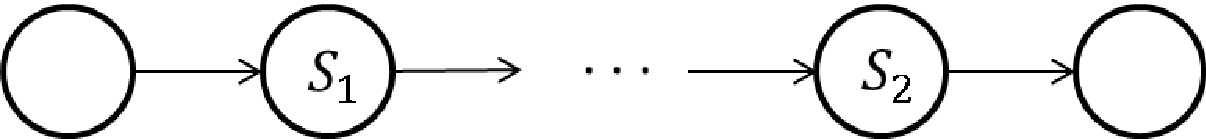
\includegraphics[width=2in]{sequence.pdf}\hfill\space\\[0.2cm]
$T=\sum\limits^m_{n=1}t_n$ \hfill $C=\sum\limits^m_{n=1}c_n$ \hfill
$A=\prod\limits^m_{n=1}a_n$ \hfill $R=\prod\limits^m_{n=1}r_n$
\end{tabular}}}
\caption{Sequence construct and calculation of its QoS properties
\cite{yu2013adaptive}.}
\label{sequence}
%\end{figure}
\vspace{0.3cm}
%\begin{figure}
\centerline{
\fbox{
\begin{tabular}{p{0.6\linewidth}}
\space\hfill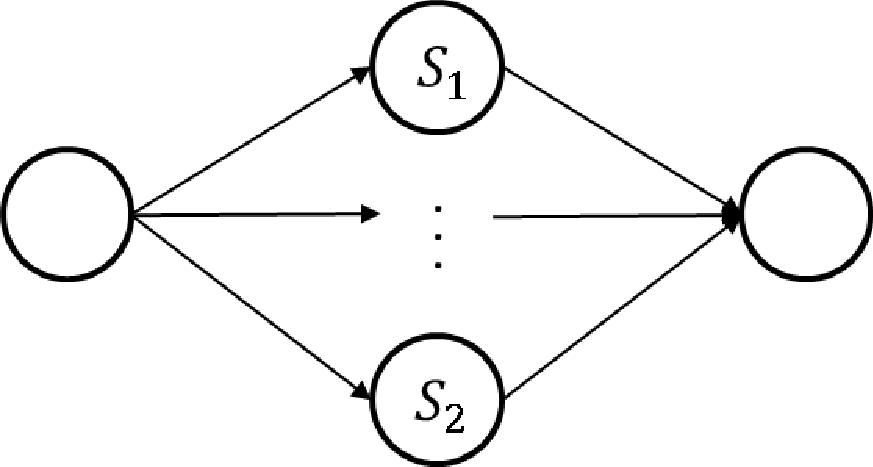
\includegraphics[width=1.4in]{parallel.pdf}\hfill\space\\[0.2cm]
\space\hfill$T=MAX\{t_n|n\in\{1,\ldots,m\}\}$\hfill\space\\[0.2cm]
$C=\sum\limits^m_{n=1}c_n$ \hfill $A=\prod\limits^m_{n=1}a_n$ \hfill
$R=\prod\limits^m_{n=1}r_n$
\end{tabular}}}
\caption{Parallel construct and calculation of its QoS properties
\cite{yu2013adaptive}.}
\label{parallel}
\end{figure}

\subsubsection{Sequence construct}
The composite web service executes each atomic service associated with a sequence construct in a definite sequence order. The aggregation value for total time ($T$) and total cost ($C$) is the sum of time and cost of web services involved respectively. The overall availability and reliability in a sequence construct are calculated by multiplying their corresponding availability and reliability of each web service in probability theory. This construct is shown in Figure \ref{sequence}.
\subsubsection{Parallel construct}
Web services in a parallel construct are executed in the meantime. The QoS aggregation value in total cost, availability and reliability are the same as these in sequence construct while the Total time ($T$) is delimited by the maximum time consumed path in the service composite solution. This construct is presented in Figure \ref{parallel}.

\subsection{Related Work} \label{relatedWork}
\textbf{Semantic web service matchmaking}. Substantial work \cite{bansal2016generalized,mier2015integrated} on semantic web service composition focused mainly on functional requirements and negect non-functional requirements. This approach utilises Description Logic($DL$) \cite{baader2003description} reasoning between input and output concepts of web services to ensure a semantic matchmaking. Since semantic descriptions are introduced into web service, which is expressed in ontologies, the semantic matchmaking is to considered be a process consisting of seeking similarity of parameters (i.e., input and output) of web services and pairing a mapping between two knowledge representations encoded utilising the ontology \cite{lecue2006formal}. In \cite{shet2012new}, the author surveyed three approaches the similarity measures using taxonomies: one is based on nodes, in which similarity is determined by the information content of the nodes; one is entirely based on edge, where concept distance in a hierarchy structure is evaluated,  and the hybrid approach that combines the previous two methods. A new similarity measure based on edge counting is introduced in a Ontology in \cite{shet2012new}, which extends similarity measure defined by Wu and Palmer \cite{wu1994verbs}. Neighbourhood concepts are considered in their model in Formular \ref{equation1}, where $\lambda$ = 1 (default value as 0).

\begin{equation}
q(s_ {similarity}){=} \frac{2N \cdot e^{-\lambda L/D} }{N_{1}+N_{2}}
\label{equation1}
\end{equation}

In \cite{lecue2009optimizing}, the quality of matchmaking problem is transferred to measure the quality of semantic links $sl_{i,j} \stackrel{.}{=} \langle s_{i}, Sim_{T}(Out\_s_i,In\_s_j),s_{j}  \rangle$, which utilise one possible measure for the degree of similarity using Common Description rate of a semantic link in Formula \ref{equation2}. And Extra Description $In_{s_{x}} \setminus Out_{s_{y}}$ and Least common subsume $lcs(Out_{s_i},In_{s_j})$ are also required to be pre-calculated in Formula \ref{equation2}. They chained the web service with five well-known matching types: Exact, Plug-in, Subsume, Intersection, and Disjoint. Therefore, the quality of the semantic link is estimated as quality criteria $q_{m}$, either 1 (Exact), 0.75 (Plugin), 0.5 (Subsume) or 0.25 (Intersection) associated with their corresponding quality of vector $q_{cd}$ defined as Formula \ref{equation3}.

\begin{equation}
q_{cd}(sl{_{i,j}})={=} \frac{|lcs(Out_{s_i},In_{s_j})|}{|In_{s_{x}} \setminus Out_{s{_y}} \stackrel{.}| +|lcs(Out_{s_i},In_{s_j})| }
 \label{equation2}
\end{equation}

\begin{equation}
\label{equation3}
q(sl{_{i,j}}) \stackrel{.}{=} (q_{mt}(sl_{i,j}), q_{cd}(sl_{i,j}))
\end{equation}

However, the weakness of this approach for semantic link quality is that calculating Extra description and Least common subsume requires well and completely defined DL in the knowledge representation system. for example, both service profiles definition described in OWL-S, and their related class, class axioms and properties defined in OWL2 are needed. This makes it nearly impossible to measure semantic matchmaking quality in most semantic web services applications. Additionally, a semi-automated service composition approach is considered by the author, rather than a fully automated method. Therefore, we introduce a more applicable evaluation model in a full automated semantic web service composition.

\textbf{QoS-aware EC approaches}. Evolution Computing techniques are widely used to solve optimisation problem. Genetic Programming (GP) \cite{da2015graphevol,da2016particle} is typical EC techniques to solve automated web service composition. GP-based approach utilises tree representations, on which service as represented as terminal nodes, and composite constructs as the functional nodes. The crossover and mutation operations reproduce various individuals while ensuring correctness of structure. In \cite{yu2013adaptive}, the author optimises the overall quality of service composition by a fitness function, which is also liable for correctness in functionality through penalising infeasible solutions. To simplify the checking of constraints for solutions, an indirect PSO-based approach was introduced in \cite{da2016particle}, firstly, the best location is looked for using PSO considering optimising QoS for building up service queue, then the web services in this service queue are selected to build up a graph representation of web service composition. However, the composite solution does not distinguish different match types and the degree of matching, which could lead to the data returned by the selected service that we think may be too general. In fact, customers' perspectives, application domains and ontology granularity all could have significant impacted on the data requested by users. In some scenarios, the output returns too broad consequences that have no meaning for the customers, even though those web services selected leads to a very good overall QoS. Therefore, we fill the gap by considering different matching types and their similarity when evaluate an overall quality of composite service.

\section{QoS-aware Semantic Automated Web Service Composition}\label{qswsc_approach}
\begin{figure}[h]
\centerline{
\fbox{
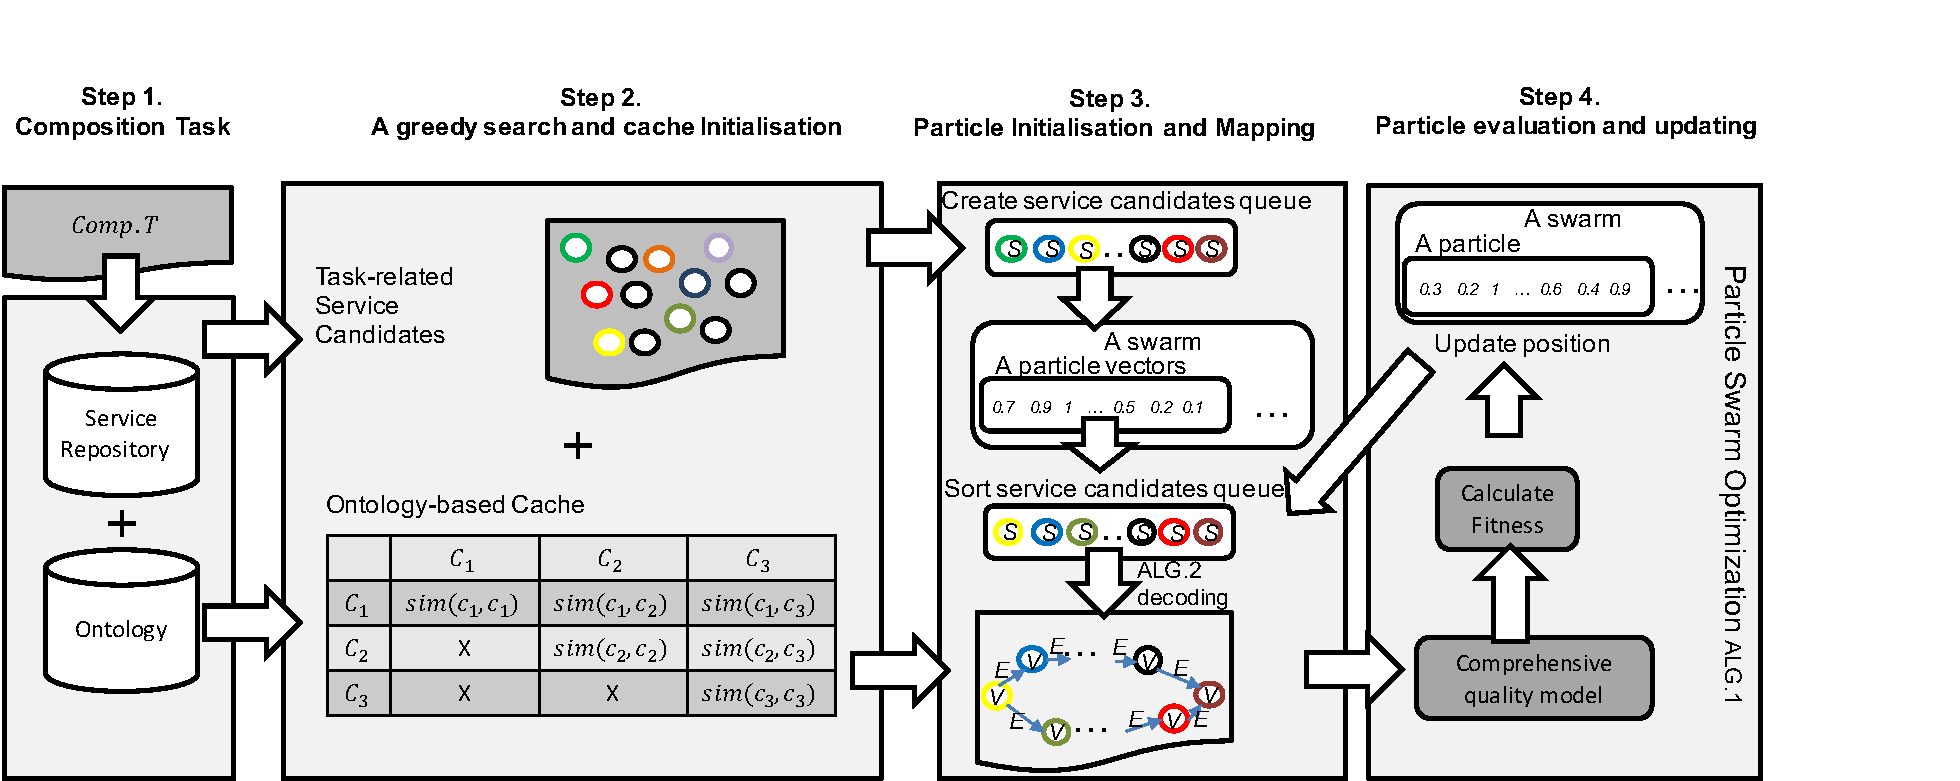
\includegraphics[width=12cm]{overview.pdf}}}
 \caption{Overview of the proposed approach.}
 \label{overview}
\end{figure}
In this paper, we model automated QoS-ware semantic service composition with graphs. PSO has shown its efficiency in solving combinatorial optimisation problems. Therefore, we will propose a PSO based approach, which is considered to be simple and efficient without penalising and repairing comparing to GP \cite{da2014graph}. Fig. \ref{overview} shows the overview of our approach with the five steps included. Step 1:The composite process is triggered by a composite goal defined in Subsection \ref{problemDes}, which describes customers requirements in terms of functional and non-functional requirement. The previous functional one is defined as $F(T_{Input}, T_{Output})$ , and the later nonfunctional one is the users' accepted level of QoS. Step 2: Those requirements are initially used to discover all relevant web services and their relationship in semantic matchmaking to get prepared for designing service composition via building graphs. This step selects relevant web services related to services request. This leads to a shrunken service repository that is used by PSO-based algorithm. Step 3: a service composition graph is randomly built up with considering the QoS and matchmaking quality. This graph building is interleaved with semantic matchmaking for services. The output of one service and its associated input of another service is calculated in the matchmaking phase where semantic matchmaking quality are measured which will be explained in Subsection \ref{qualityModel}. Step 4,5: The optimisation of service composition solution is performed over the PSO in Section \ref{pso_algorithm}, which is used to find optimised particle locations mapped back to web service for service-graph building. This approach \cite{da2016particle} is an indirect representation of web service composition that constructing a graph-based composite service composition.
\subsection{Semantic matchmaking}
The semantic matchmaking is achieved by utilising semantic annotation with OWL and OWL-S. In this paper, we use MECE ontologies \cite{bleul2008self} XWL format, which could be considered to be an alternative form of ontology for services. In OWL, semantics specifies the both concepts and individuals in the forms of classes and instances but limited to taxonomies. The semantic concepts are expressed with the their statements and relationship in RDFs (such as subClassOf ), and the semantic individuals are related to the input and output parameters of web services. The MECE is an extensive annotation to WSDL files, which defines the each parameter of services associated with their semantic individuals. The overall matching making process is demonstrated in Figure \ref{matchmaking}.

\begin{figure}[h]
\centerline{
\fbox{
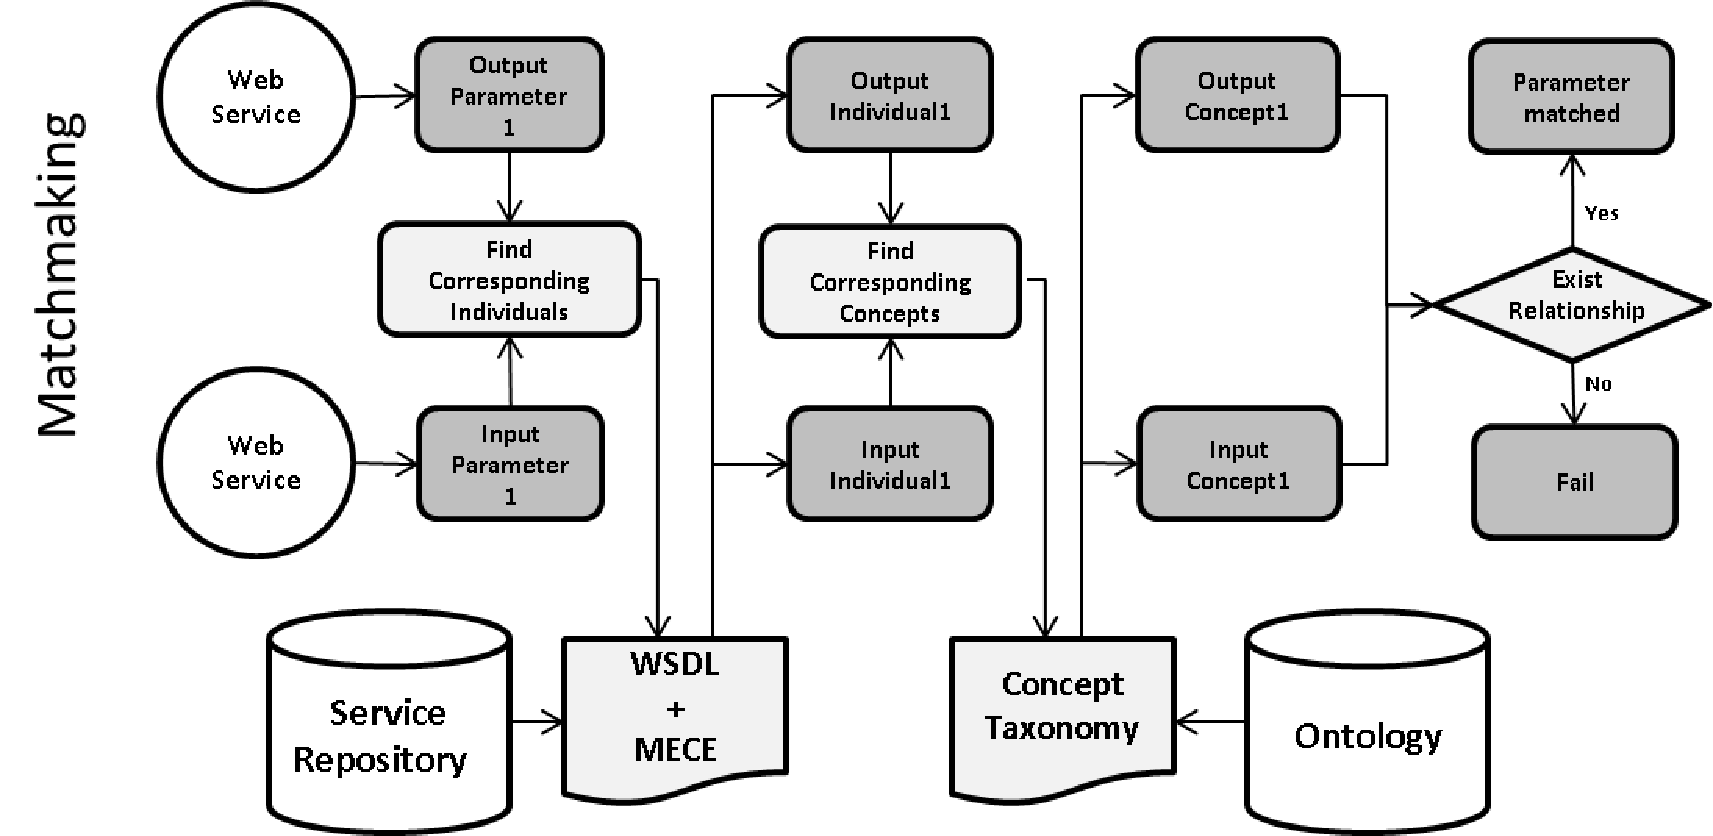
\includegraphics[width=10cm]{matchmaking.pdf}}}
 \caption{Semantic matchmaking.}
 \label{matchmaking}
\end{figure}

The semantic matchmaking transfer a function match between $S_{1}: S_{output} \in C_{1}$ and $S_{2}:S_{output} \in S_{b}$ to a pair of concept match: $match(C_{2}, C_{3})$ defined in Section \ref{semantic Web service Discovery}. The matching mechanism attempts to determine whether correct match criteria between the source concepts of C1 and the target concepts of C2, and the quality of semantic matchmaking for these two concepts is calculated in the quality model in subSection \ref{qualityModel}. The advantage of utilising semantic matchmaking quality is to find a more closely requested service output with acceptable level of QoS.

\subsection{Comprehensive quality model and aggregation matrix}\label{qualityModel}
In this paper, we propose a semantic matchmaking model to evaluate the semantic quality of two matched web services, this fill the gaps in subsection \ref{relatedWork} of current prevailing QoS-aware optimisation, where quality of matchmaking for service selection are not considered.

\textbf{Semantic matchmaking model}. Due to the discretisational characteristics of different match types, which is driven by the cost of  data type integration and manipulation \cite{lecue2009optimizing}. Match type is considered to be one factor for the semantic quality. Another factor in our proposed model is concept similarity, which could be evaluate based on edge counting method defined by \cite{shet2012new}, a taxonomy based measurement for ontology matching, In this paper, it could be used to estimate the parameter concepts similarity between the output and input of a request for selecting web services with close semantic matching. Therefore, given the quality match type and the similarity of two parameters, the semantic matchmaking quality is defined as Formula \ref{equation4}, where $q(s_ {matchType})$ is set up as the same as the quality of the semantic link in literature \cite{lecue2009optimizing} as 1 (Exact), 0.75 (Plugin), 0.5 (Subsume) or 0.25 (Intersection) while $q(s_ {similarity})$ is calculated utilising formula \ref{equation1} in subsection \ref{relatedWork}.

\begin{equation}
\label{equation4}
q_{smq} \stackrel{.}{=} (q(s_ {matchType}), \  q(s_ {similarity}))
\end{equation}

\textbf{Comprehensive quality model}. Compared to QoS evaluation model, the comprehensive quality model is established to investigate both functional and non-functional requirements of composite web services. The non-functional properties typically refer previously discussed QoS, which are given by service providers. Consequently, the comprehensive quality model integrated the semantic matchmaking quality $q(s_{smq})$ in Formula \ref{equation5}, which could be further broken down into Formula \ref{equation6}.

\begin{equation}
\label{equation5}
q_{cq} \stackrel{.}{=} (q(s_ {smq}), \  q(s_ {QoS}))
\end{equation}
\begin{equation}
\label{equation6}
q_{cq} \stackrel{.}{=} (q(s_ {mt}), \  q(s_ {s}), \  q(s_{a}),\  q(s_{r}),\  q(s_{c}),\  q(s_{t}))
\end{equation}

\textbf{Quality aggregate matrix}.The quality aggregation is defined based on the constructs of composite web services on the criteria of functional and non-functional properties. Typically, web services could have more than one concept-related parameters. Regarding semantic matchmaking part, edge-level quality aggregation is determined by the mean of concept-related parameter quality in both semantic match type and similarity respectively, and construct-level quality is further calculated based on the edge-level quality aggregation following the rules in Table \ref{table1}, which is the quality aggregate matrix for semantic web service composition. Semantic matchmaking aggregation considers two different factor aggregations: the matching type quality aggregation is calculated by the product function of involved edge-level matching type value, and the similarity quality average value of all edge-level similarity quality. The nonfunctional (QoS) aggregation calculation is same to \cite{cardoso2004quality}.

% Please add the following required packages to your document preamble:
% \usepackage{multirow}
\begin{table}[]
\centering
\caption{Quality aggregate matrix for semantic web service composition}
\label{table1}
\begin{tabular}{|c|c|c|c|l|}
\hline
\multicolumn{3}{|c|}{Composition Construct}                                      & Sequence                             & Parallel \\ \hline
\multirow{5}{*}{QualityFactors} & \multirow{2}{*}{Functional}    & $Q(s_ {mt})$  &$\prod_{n=1}^{m} q(s_ {mt})$          &  $\prod_{n=1}^{m} q(s_ {mt})$ \\ \cline{3-5}
                                &                                & $Q(s_ {s})$  & $(\sum_{n=1}^m q(s_ {s}))/m$        &  $(\sum_{n=1}^m q(s_ {s}))/m$  \\ \cline{2-5}   
                                & \multirow{4}{*}{NonFunctional} & $Q(s_{a})$    & $\prod_{n=1}^{m} q(s_a)$             &  $\prod_{n=1}^{m} q(s_a)$ \\ \cline{3-5} 
                                &                                & $Q(s_{r})$    & $\prod_{n=1}^{m} q(s_r)$             &  $\prod_{n=1}^{m} q(s_r)$ \\ \cline{3-5} 
                                &                                & $Q(s_{c})$    & $\sum_{n=1}^m q(s_ {c})$             &  $\sum_{n=1}^m q(s_ {c})$ \\ \cline{3-5} 
                                &                                & $Q(s_{t})$    & $\sum_{n=1}^m q(s_ {t})$             &  $max(q(s_ {t}))$ \\ \hline
\end{tabular}
\end{table}

\subsection{Fitness Calculation}
The fitness value is calculated from the aggregate value of quality components involved in a graph-based service composition. A weighted sum of those components is utilised in the fitness function \ref{equation7}, in which fitness value of 1 means the best overall quality and 0 means the worst. As the sum of all the function weights (w1 to w6) is equal to 1, $MT$, $S$, $A$, $R$, $T$, and $C$ must be normalised ranging from 0 to 1 so that the overall result falls within 0 to 1. Also, the lowest T and C value represent the best quality so that the objective function is offset using $(1 - T)$ and $(1 - C)$.

\begin{equation}
\label{equation7}
Fitness = w_1MT + w_2S + w_3A + w_4R + w_5(1 - T) + w_6(1 - C)
\end{equation}

\noindent where $\sum_{i=1}^{6} w_i = 1$


\subsection{QoS-aware Semantic Web Service Composition algorithm} \label{pso_algorithm}
\begin{algorithm}[!htb]
 \setlength\hsize{0.9\linewidth}
 \SetKwInOut{Input}{Input}\SetKwInOut{Output}{Output}
 \let\oldnl\nl% Store \nl in \oldnl
\newcommand{\nonl}{\renewcommand{\nl}{\let\nl\oldnl}}
\textbf{Input}: I, O \\
\textbf{Output}: G \\
 \LinesNumbered
	\textbf{1.} Randomly initialise each particle in the swarm.\\
	\nonl \While {max. iterations not met}{
		\ForAll{particles in the swarm}{
			\textbf{2.} Sort particle's position vector as a service queue in ascending order\\
			\textbf{3.} Initialise OutputSet with Task Input: I\\
			\textbf{4.} Initialise a graph G with a startNode\\
			\nonl \While {max. OutputSet not contains Task Output: O}{
				\textbf{5.} Get web service from service queue\\
				\If{All inputs of current web service satisfied with output from outputSet}{
					\textbf{6.} Create and connect service edge associated with matchmaking quality to graph.\\
					\textbf{7.} Create and connect node(current web service) to graph.\\
					\textbf{8.} Remove current web service from the queue.\\
					\textbf{9.} Update OutputSet with outputs current web service.\\
				}
				\textbf{10.} Get next web service from service queue\\
			}
			\textbf{11.} Connect endNode the graph G\\
			\textbf{12.} Remove dangle services from the graph G\\
			\textbf{13.} Remove dangle edges from graph G\\
			\textbf{14.} Aggregation of semantic matchmaking and QoS\\
			\textbf{15.} Calculate the particle's fitness.\\
			\eIf{fitness value better than pBest}{
				\textbf{16.} Assign current fitness as new pBest.\\
			}{
				\textbf{17.} Keep previous pBest.\\
			}		
		}
		\textbf{18.} Assign best particle's pBest value to gBest, if better than gBest.\\
		\textbf{19.} Calculate the velocity of each particle according to the equation:\\
		\textbf{19.} Update the position of each particle according to the equation:\\
	}
	
 \caption{Steps of graph-based PSO optimisation technique.}
\label{psoSteps}
\end{algorithm}
The overall algorithm investigated here is a combination of a simple forward decoding PSO \cite{da2016particle} with our comprehensive quality evaluation model. The idea is to translate the particle location into a service queue as an indirect representation of service composition graph, finding the best fitness of the composite service solution is to discover the optimised location of the particle. In PSO, the dimension of the particle is set up as the same as the number of relevant web services in the shrunken service repository, each of which is mapped to a location in a particle, put services in a queue and sort in ascending order. Later on, we decode a corresponding graph built from that service queue using a forward graph-building technique from a start node to the end node. We select and connect web services to the startNode if this web service can satisfy the given Task input, and an Output Set is initialised and kept updating with outputs from new added web services in the graph, later on, we services are keeping being selected and added if services' inputs could be satisfied by any output in the Output Set, if the Output Set contains the Task's required outputs, we end up graph building. In addition, dangle service nodes and edges should be removed. At last, fitness value can be calculated by the construct-based aggregation.



\section{Experiment Design}\label{experiment_design}
In this section, a quantitative evaluation approach is adopted in our experiment design. The objectives of the evaluation are to measure the effectiveness of the proposed comprehensive quality model in automated semantic web service composition approach, and to explore the impact of the semantic matchmaking that contributes to overall composition quality, and to compare solutions generated by QoS-ware approach with our method.

We utilise benchmark dataset web service challenge 2009 (WSC09) \cite{kona2009wsc} web service data sets to perform a standard evaluation. WSC09 designed OWL for providing richer semantics consisting tasks with variable size. With an incremental number in concept, individuals and web services in each dataset, it is a proper dataset for the scalability measures in our defined quality evaluation model. Table \ref{wsc09datasetTable} presents the features of the WSC’09 dataset. The number of concepts, individuals in the ontology and services of each data set is shown in the second, third, fourth column respectively. Also, we extend all the datasets with QoS attributes from service providers to perform a comprehensive quality evaluation. 
\begin{table}[]
\centering
\caption{Features of the WSC09 datasets}
\label{wsc09datasetTable}
\begin{tabular}{|l|l|l|l|}
\hline
\multicolumn{1}{|c|}{Dataset} & No.Concept & No.Individual & No.Service \\ \hline
WSC09 01                     & 1578       &3102           &572      \\ \hline
WSC09 02                     & 12388      &24815          &4129      \\ \hline
WSC09 03                     & 18573      &37316          &8138      \\ \hline
WSC09 04                     & 18673      &37324          &8301      \\ \hline
WSC09 05                     & 31044      &62132          &15211    \\ \hline
\end{tabular}
\end{table}


We run the experiment under computing grid comprising of almost 170 NetBSD (Unix operating system) workstations operated by the Sun Grid Engine. Experimentation was done using the approach explained in Section \ref{qswsc_approach}, and evaluated in the comprehensive quality model introduced in Subsection \ref{qualityModel}. The parameters were chosen based on general settings from \cite{shi2001particle} for our PSO-based approach, 30 particles evolved in 100 generations in the searching space, in which problem dimension's size equals to the relevant service size shown in graph. we run 30 times independently for each dataset. In addition, weights setting are flexibly defined by users' preferences. As part of their requirement, we configure weights of fitness function as the same to properly balance functional side and nonfunctional side. Therefore, $w_{1}$ and $w_{2}$ are equals to 0.1 and 0.4,  and $w_{3}$, $w_{4}$, $w_{5}$, $w_{6}$ are all set to 0.125 accordingly.

\section{Results and Analysis}\label{results_analysis}
\subsection{Convergence Test}\label{convergenceTest}
To analysis the effectiveness of our approach, we explore the convergency rate of the proposed method in this section. We show the convergency of five tasks in WSC09. To further study an overall effectiveness of evaluation model and investigate the impacts of all involved components in the fitness function. We analysis all the performance of these components in the whole evolutionary process in Figure \ref{exp_fitnessvalue}, in which the five tasks' experiment results are arranged in four groups consisting of average fitness, average matchType quality, average similarity quality and average quality of service for generation 0-99 with optimum.
\begin{figure}[h]
\centerline{
\fbox{
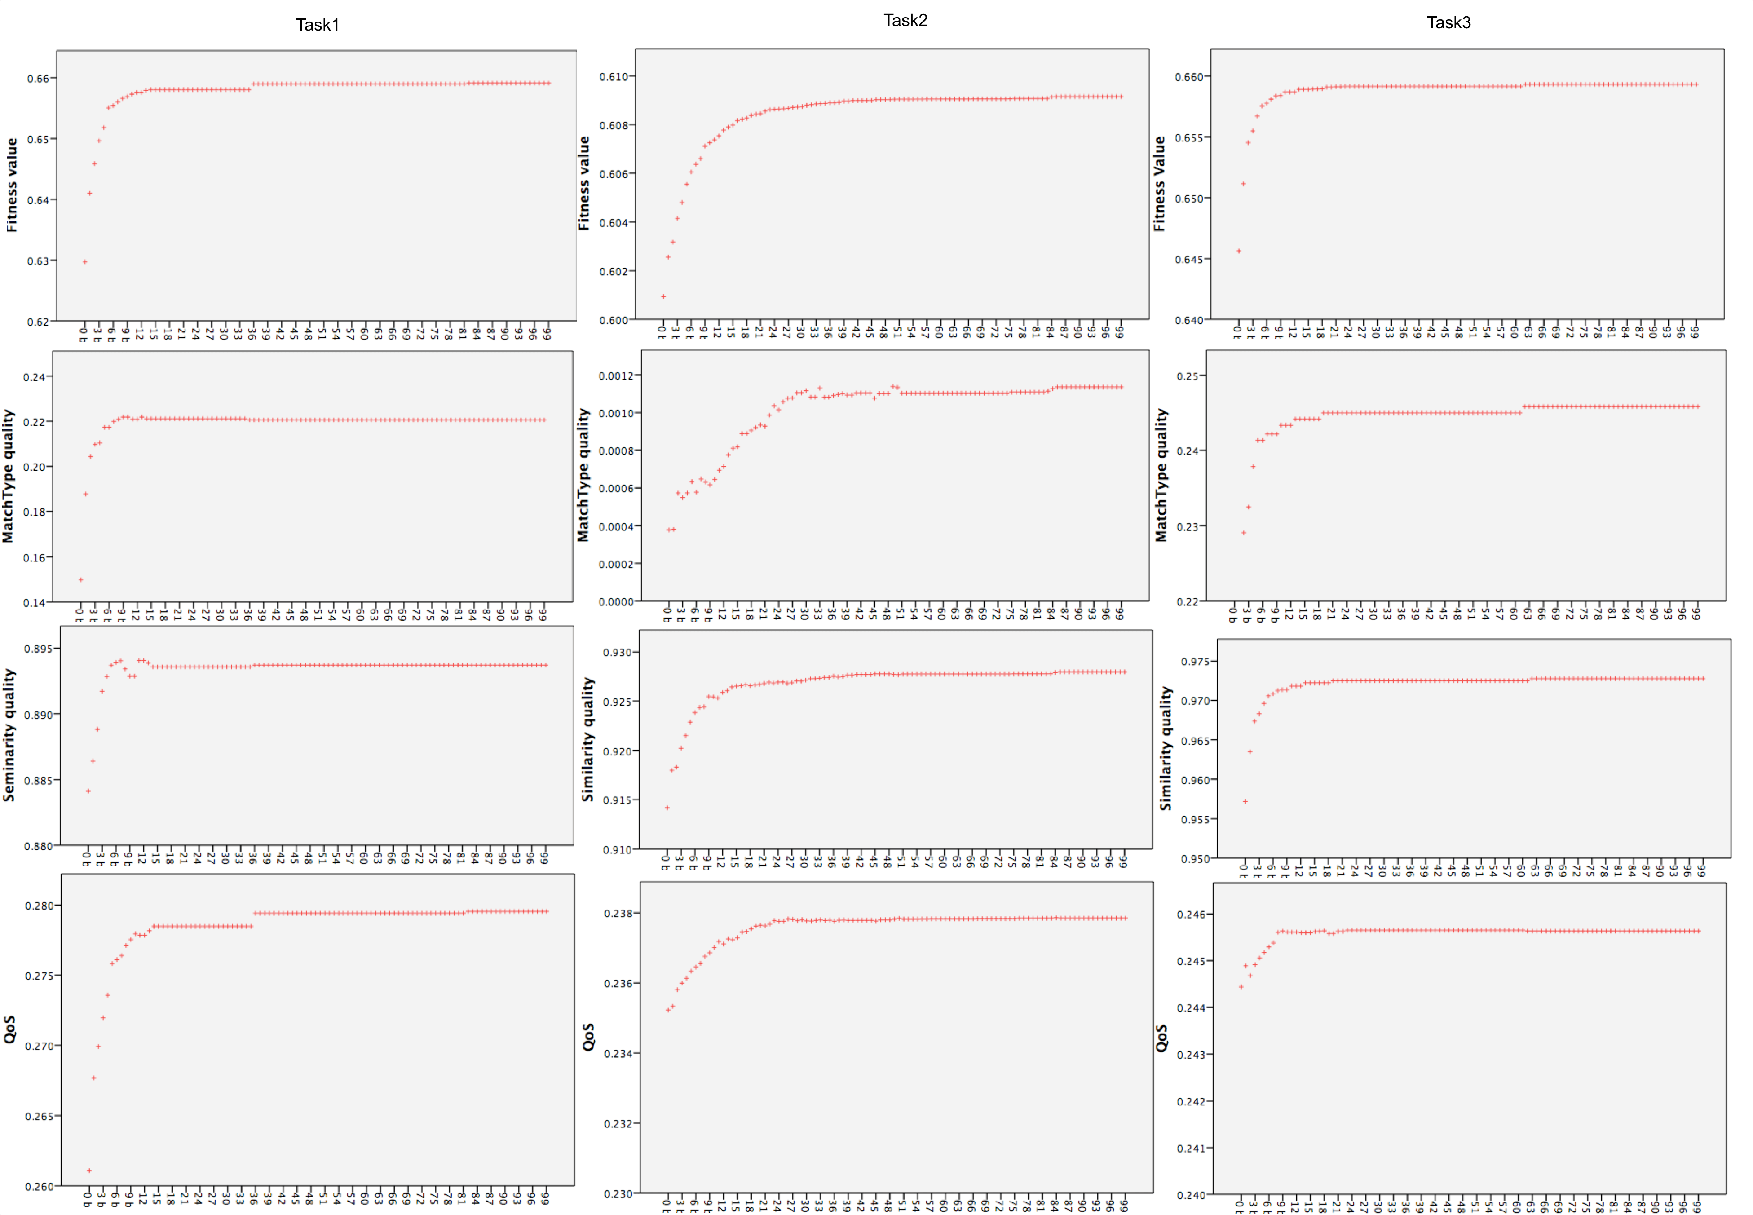
\includegraphics[width=12cm]{convergency.pdf}}}
 \caption{Average Fitness, Average MatchType Quality, Average Similarity quality and Average QoS per generation with comprehensive quality optimum}
 \label{exp_fitnessvalue}
\end{figure}

Firstly, the average fitness value over 100 generations is calculated by the average best fitness so far found per generation over 30 independent runs. The value plotted in the first column group of figure \ref{exp_fitnessvalue} ranges from 0 to 1, and it is considered to be more optimised if its value is closer to value 1. We can see that there is a significant increase in the fitness value (avg) with optimum between generation 0 and generation 15-25, the remained generation continues to produce a steady but moderate improvement in the fitness value and eventually reach a plateau with no further changes. The same behaviour is observed over the rest tasks. Also, there is a fast convergence of the fitness value can be observed. That is simply because of many repetitive solutions as the indirect web service composition representation in a large search space.

We also investigate the variation in functional quality part including two sub factors --- average matchType quality and average similarity quality from generation 0 to 99 in second and third column groups in Figure \ref{exp_fitnessvalue}. In these groups,  both the average matchType quality and average similarity quality are the average value corresponding to the average best fitness so far found plotted in the first column group,  and further calculated their mean over 30 independent runs respectively. The dominant tendency of the marked value representing a similar characteristic compared to the average fitness value group trend. However, there are some slight fluctuations over the generations, and it could be reasonably treated as a typical situation that theoretically single objective function prevents selecting the lowest semantic matchmaking quality without granting for the excellent.

Lastly, It is interesting to look at the average QoS per generation for the 30 independent runs if the behaviour of functional part performance is towards a higher value, where QoS is the value corresponding to the best fitness so far found in each generation. We construct the results in the fourth column group in Figure \ref{exp_fitnessvalue}. It is obvious that the overall trend of QoS moves upward to a high constant level in five independent tasks. Additionally, QoS (avg) with optimum have evolved towards an overall excellent state, because we don't see too much trade-off from QoS regarding the improvement in functional quality part. 

\subsection{Comparision Test}\label{comparisionTest}
\begin{figure}[h]
\centerline{
\fbox{
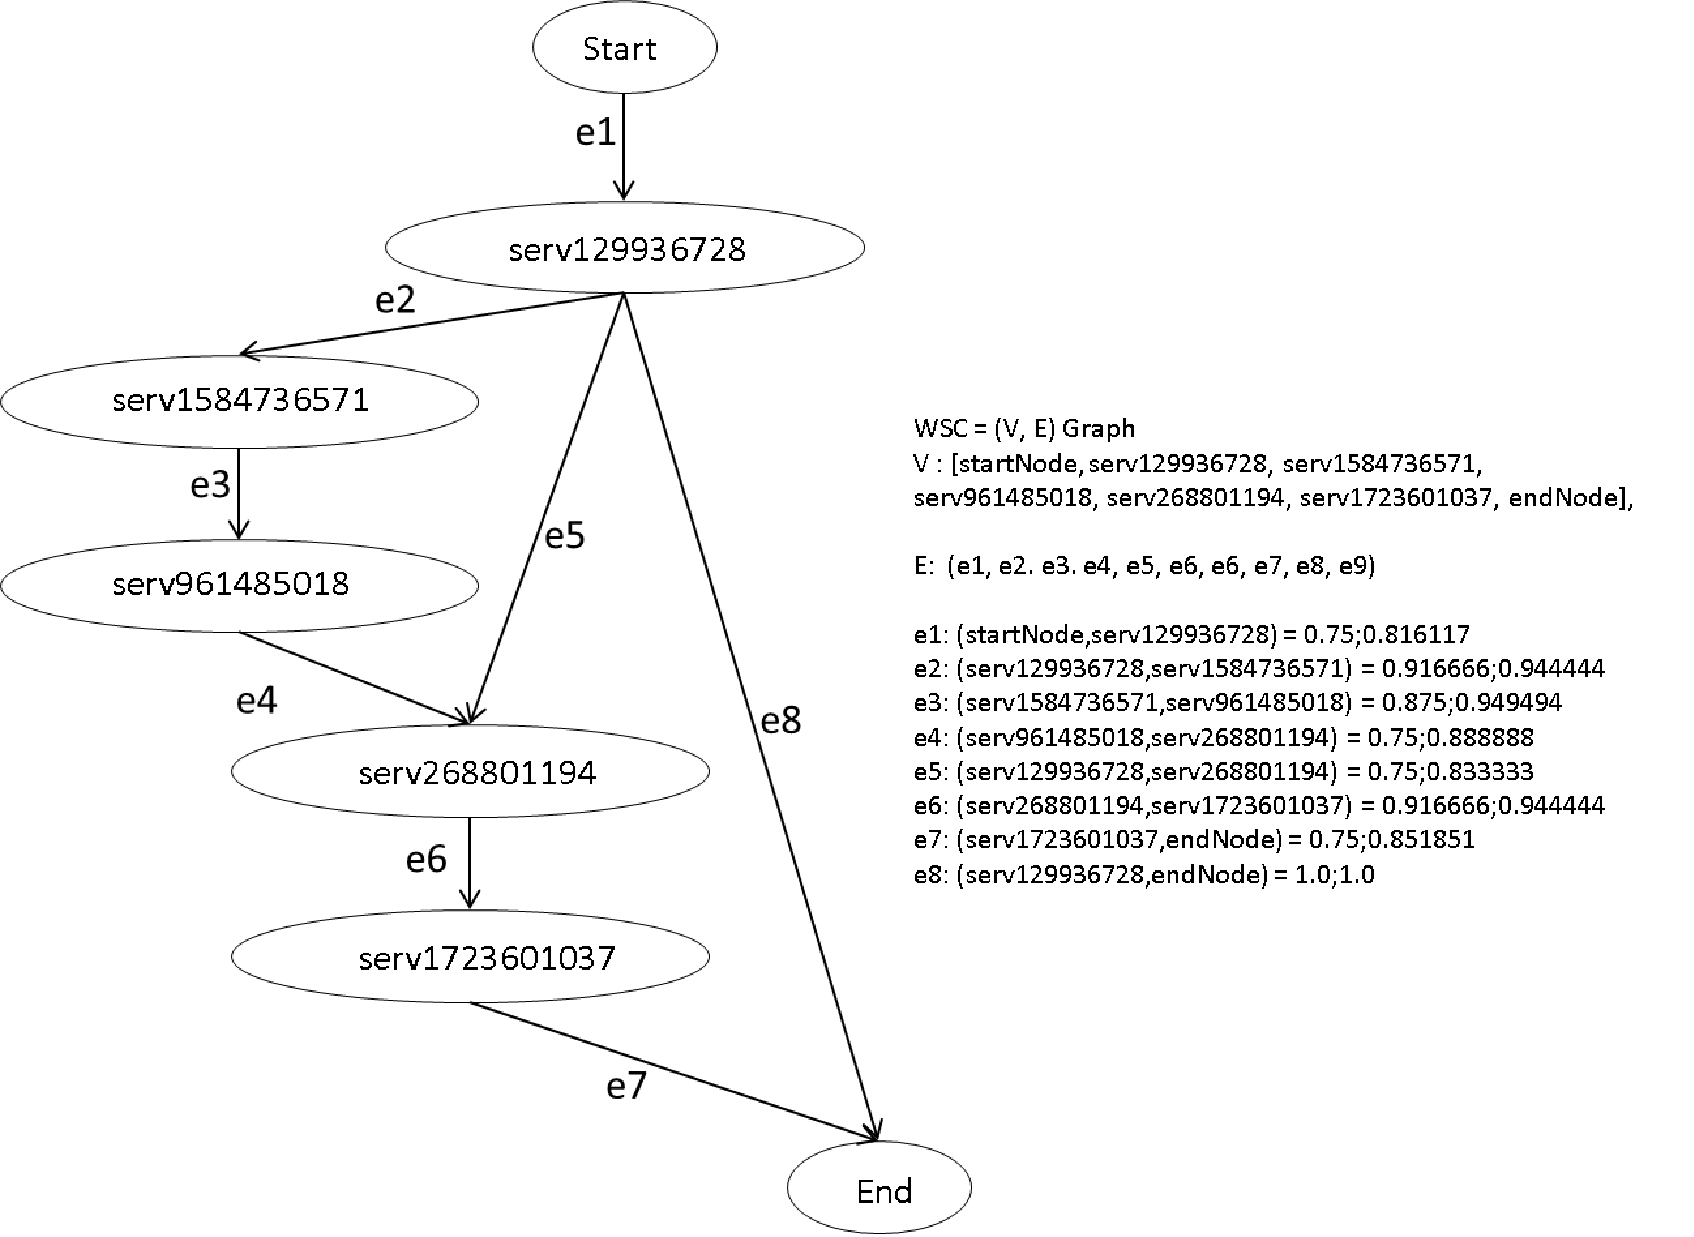
\includegraphics[width=8cm]{wscs.pdf}}}
 \caption{Example composition solutions for problem1 WSC'09.}
 \label{wscs}
\end{figure}
We defined our optimised web service composition as $WSC = (V, E)Graph$, where $V$ is a set of services as vertex: $V=[S1, S2...Sn]$ and $E$ is a set of service connections as edges associated matchType quality and semantic similarity quality: $E = {e_{1}, e_{2},... e_{n}}$ where $e1$ is define as $(S_{1},S_{2})={q_{mt}, q_{s}}$. Here we provide an example of the web service composition solution to task 1, which can be described in the Figure \ref{wscs}. The data of composite web service flows from the start to the end, where five web services involved and linked with each other using edge connections. Besides that, $q_{mt}$ and $q_{s}$) are calculated for all edges ${e_{1}, e_{2},... e_{n}}$, and further aggregated in $Q_{mt}$ and $Q_{s}$ respectively.In addtion, $Q_{QoS}$ is calculated by all the non-functional attributes of $V$ using aggregation rules defined before.This standard solution model helps us to make better comparison for evaluating the results from different approaches.

After a well-defined solution is discussed, we will look at $Q_{mt}$, $Q_{s}$ and $Q_{QoS}$ defined in the solution model using black-box testing for solution comparison, where these components in both comprehensive quality evaluation approach and traditional QoS-ware one \cite{feng2013dynamic,huang2009effective,ma2015hybrid,da2014graph} are compared to reveal how good our evaluation mode is. In a decision table \ref{decisionTable}, optimised solution using these two evaluation models are compared under five independent tasks in WSC09 dataset. In each task solution, we compare $Q_{mt}$,$Q_{s}$ and $Q_{QoS}$, where $Q_{QoS}$ is normalised to make them comparable from 0 to 1 in our method. 

% Please add the following required packages to your document preamble:
% \usepackage{multirow}
\begin{table}[]
\footnotesize
\centering
\caption{Quality of two evaluation model in a decision table}
\label{decisionTable}
\begin{tabular}{|c|c|c|c|}
\hline
\multicolumn{2}{|c|}{\multirow{2}{*}{}}                              &Approach 1           &Approach 2                           \\ \cline{3-4} 
\multicolumn{2}{|c|}{}                                               & \shortstack{QoS-aware \\ Evaluation} & \shortstack{Comprehensive \\ Quality Evaluation} \\ \hline
\multirow{3}{*}{Condition}            & dataset1             & $\surd$              & $\surd$                            \\ \cline{2-4} 
                                      & dataset2             & $\surd$              & $\surd$                            \\ \cline{2-4} 
                                      & dataset3             & $\surd$              & $\surd$                            \\ \hline
\multirow{3}{*}{\shortstack{Task1\\Optimised solution}}  &$Q_{mt}$   & .232635              & .232635                          \\ \cline{2-4} 
                                      &$Q_{s}$                       & .903572              & .903572                          \\ \cline{2-4}
                                      &$Q_{QoS}$                     & .578577              & .578577                          \\ \hline
\multirow{3}{*}{\shortstack{Task2\\Optimised solution}}  &$Q_{mt}$   & .001828              & .000851$\downarrow$               \\ \cline{2-4} 
                                      &$Q_{s}$                       & .917172              & .938840$\uparrow$                 \\ \cline{2-4}
                                      &$Q_{QoS}$                     & .480251              & .473002$\downarrow$               \\ \hline
\multirow{3}{*}{\shortstack{Task3\\Optimised solution}}  &$Q_{mt}$   & .191188              & .247836$\uparrow$                  \\ \cline{2-4} 
                                      &$Q_{s}$                       & .951509              & .973723$\uparrow$                  \\ \cline{2-4}
                                      &$Q_{QoS}$                     & .493927              & .491538$\downarrow$                 \\ \hline
\multirow{3}{*}{\shortstack{Task4\\Optimised solution}}  &$Q_{mt}$   & .919678              & .943406$\uparrow$                  \\ \cline{2-4} 
                                      &$Q_{s}$                       & .000000              & .000009$\uparrow$                  \\ \cline{2-4}
                                      &$Q_{QoS}$                     & .480818              & .472485$\downarrow$                 \\ \hline
\multirow{3}{*}{\shortstack{Task5\\Optimised solution}}  &$Q_{mt}$   & .000094              & .000109$\uparrow$                  \\ \cline{2-4} 
                                      &$Q_{s}$                       & .927476              & .930975$\uparrow$                  \\ \cline{2-4}
                                      &$Q_{QoS}$                     & .476236              & .475128$\downarrow$                 \\ \hline                                                   
\end{tabular}
\end{table}
From the table \ref{decisionTable}, Task 1 represents the same solution that can be observed in values of  $Q_{mt}$,$Q_{s}$ and $Q_{QoS}$ using the smallest dataset size with the lowest size of ontologies. However, we can recognise trade-offs in task2 and task3 using our evaluation model, where a 0.021668 increase and a 0.00098 decrease in similarity quality and matchType quality with weights 0.4 and 0.1 respectively so that solution to task 2 is still considered to be an improvement in functional quality part with a trade-off value 0.007249 in QoS. In task3, the benefit of functional part quality is clearer with an increase in both similarity quality and matchType quality of 0.056648 and 0.078862 while a slight decrease in QoS. later on, the performance is the same in task 4 and task 5. In conclusion, we can perceive that our evaluation could find out better functional quality with a reasonable trade off in QoS.

\section{Conclusion}\label{conclusion}
This work introduced a more applicable and simpler evaluation model for semantic automated web service composition that relies on semantic matchmaking quality extension to QoS-aware consideration. The key idea of these evaluation model is to consider the quality of semantic matchmaking corresponding to different matchmaking types, which is simply achieved by applying the similarity measures in parameter-related concepts, and those web services are involved in further selection for dealing optimised problems. Also, the effectiveness of our model is also proved to be able to obtain a better-optimised solution in better functional quality with a reasonable trade-off in QoS. Future works in this area should investigate in multi-objective optimisation as well as consider improving efficiency in the functional quality calculation.
\bibliographystyle{splncs03}
\bibliography{bibliography}

\end{document}